\documentclass{ximera}

\begin{document}

\begin{question}
  Find 
  \[
  \displaystyle \lim_{x\to \pi/2} f(x)
  \]
  where
  \[
  f(x) = \left\{\begin{array}{cl} \sin x & x\leq \pi/2, \\ \cos x & x>\pi/2. \end{array}\right.
  \]
  \begin{solution}
    \begin{hint}
     Both $\sin x$, for $x\leq\pi/2$, and $\cos x$, for $x>\pi/2$ are continuous on their respective domains. However, for the limit $\lim\limits_{x\to\pi/2}f(x)$ to exist, both the left-hand and the right-hand limits must exist and be equal.
    \end{hint}
     \begin{hint}
    	Take a look at the graph of the function
    \begin{center}
     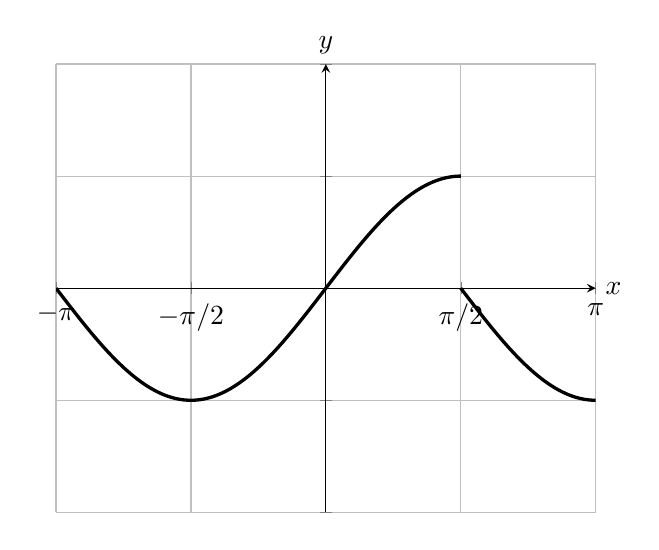
\begin{tikzpicture}
	\begin{axis}
	[ymin=-2,ymax=2, axis lines=center,xlabel=$x$,ylabel=$y$,every axis y 
	label/.style={at=(current axis.above origin),anchor=south},every axis x label/.style={at=(current axis.right of origin),anchor=west},
	domain=-pi:pi,
	yticklabels={},
	xtick={-3.141592653589793,-1.570796326794897,0,1.570796326794897,3.141592653589793},
	xticklabels={$-\pi$,$-{\pi}/{2}$,$0$,${\pi}/{2}$,$\pi$},
	ymajorgrids=true,
	grid = major
	]
	\addplot[domain=-pi:pi/2,very thick,smooth,samples=1000]
	{sin(deg(\x))};
	\addplot[domain=pi/2:pi,very thick,smooth,samples=1000]
	{cos(deg(\x))};
	\end{axis}
       \end{tikzpicture}      
      \end{center} 
    \end{hint}
    \begin{hint}
     Evaluating $\lim\limits_{x\to{\pi/2}^{+}}f(x)$ we see that it tends to $\cos \pi/2=0$. This follows because, for $x>\pi/2$, we are on the piece of $f(x)$ given by $\cos x$ and the limit $\lim\limits_{x\to{\pi/2}}\cos x=0$, certainly. On the other hand, evaluating $\lim\limits_{x\to{\pi/2}^{-}}f(x)$ we see it tends to $\sin \pi/2=1$. This follows because, for $x\leq\pi/2$, we are on the piece of $f(x)$ given by $\sin x$ and the limit $\lim\limits_{x\to\pi/2}\sin x=1$, certainly. These are not equal.
    \end{hint}
     The 
    \answer{\text{limit does not exist}}.
  \end{solution}
\end{question}

\end{document}